\documentclass{report}
\usepackage{graphicx} % Required for inserting images
\usepackage{amsmath}
\usepackage{amssymb}
\usepackage{multirow}
\usepackage{placeins}
\usepackage{cancel}
\usepackage{minted}
\usepackage{hyperref}
\usepackage{listings}
\usepackage{xcolor}

\lstset{
  language=Python,
  basicstyle=\ttfamily\small,
  keywordstyle=\color{blue!70!black}\bfseries,
  commentstyle=\color{green!50!black}\itshape,
  stringstyle=\color{orange!80!black},
  numberstyle=\tiny\color{gray},
  numbersep=8pt,
  showstringspaces=false,
  breaklines=true,
  frame=single,
  rulecolor=\color{gray!40},
  backgroundcolor=\color{gray!5},
  tabsize=2,
  captionpos=b,
}
\usepackage[natbib=true]{biblatex}
\addbibresource{bib.bib}

% Underline figure-panel labels (Left/Right/Centre/...) so captions are easy to scan.
\newcommand{\panel}[1]{\underline{#1}}

\begin{document}

\begin{titlepage}
\centering

% Logo: drop the official mark at thesis/polito_logo.pdf (preferred) or .png and it
% appears automatically; the page builds fine without it.
\IfFileExists{polito_logo.pdf}{%
  
\includegraphics[height=2.4cm]{polito_logo.pdf}\par\vspace{0.9cm}}{%
  \IfFileExists{polito_logo.png}{%
    
\includegraphics[height=2.4cm]{polito_logo.png}\par\vspace{0.9cm}}{\vspace{0.4cm}}}

{\scshape\LARGE Politecnico di Torino\par}
\vspace{0.45cm}
{\scshape\large Master's Degree in Physics of Complex Systems\par}
\vspace{0.2cm}
{\large\itshape Master's Thesis\par}

\vspace{1.6cm}
{\color{gray!55}\rule{\linewidth}{0.4pt}}\par
\vspace{0.7cm}
{\huge\bfseries Can a simple model explain economics?\par}
\vspace{0.7cm}
{\color{gray!55}\rule{\linewidth}{0.4pt}}\par

\vspace{2cm}
\begin{minipage}[t]{0.46\textwidth}
  \raggedright\large
  {\scshape\normalsize Candidate}\par\vspace{0.25cm}
  Ludovico Furlanetto
\end{minipage}\hfill
\begin{minipage}[t]{0.46\textwidth}
  \raggedleft\large
  {\scshape\normalsize Supervisors}\par\vspace{0.25cm}
  Fabi{\'a}n Aguirre-L{\'o}pez\\
  Luca Dall'Asta
\end{minipage}

\vfill
{\large July 2026\par}
\vspace{0.25cm}
{\normalsize Academic Year 2025/2026\par}
\end{titlepage}




\begin{abstract}
Firm growth shows two robust anomalies: the volatility of a firm's growth rate falls
with size far more slowly than independence would predict, $\sigma(S)\sim S^{-\beta}$
with $\beta\approx0.15$--$0.20$ rather than $1/2$, and the growth-rate distribution is
sharply peaked and fat-tailed rather than Gaussian. The standard explanations place the
source inside each firm, in a heavy-tailed composition of internal sub-units, a granular
picture that \citet{moran2024} test against firm data and find fails; the missing
ingredient, they argue, is correlations that grow with a firm's size. We ask instead
whether a dynamical model of interacting firms can generate both facts on its own, without
external noise.

We model the economy as a Generalized Lotka--Volterra system on a sparse random graph, in
which the interactions act on a firm's size relative to the average firm rather than on
its absolute size. This makes the dynamics
scale-invariant, so the economy grows, while in the strongly disordered regime its
composition never settles but keeps churning. In this persistently fluctuating state the
two anomalies emerge together as stationary properties of the interactions. The
size--variance exponent comes out about four times too steep, $\beta\approx0.8$. Its
higher moments reproduce the anomalous multiscaling the granular
picture cannot, the growth-rate distribution is symmetric and fat-tailed, and the heavy
tails persist among the largest firms.
\end{abstract}

\clearpage
\tableofcontents

\chapter{Introduction}

A well-known stylized fact about firms is how the volatility of their growth rate
depends on their size. If you measure how much a firm's growth
rate fluctuates from year to year, this volatility falls with size as $\sigma(S) \propto S^{-\beta}$, and in the data the
exponent is $\beta \approx 0.15$--$0.20$ \citep{stanley1996,
amaral1997}. Alongside this scaling, the growth-rate distribution is sharply peaked and
fat-tailed rather than Gaussian. The standard way to explain both facts is the
granular mechanism of \citet{wyartbouchaud2003} and \citet{gabaix2011}: a firm's
activity is concentrated in a few large sub-units rather than spread evenly across
many comparable ones, so a handful of dominant parts produce most of its
fluctuations, and the volatility decreases only slowly as the firm grows. Recently,
however, \citet{moran2024} confronted these models with firm data and found that they
do not hold: the size-conditioned volatility distribution has a tail far too thin to
match the granular prediction, and the growth rates stay fat-tailed even after
rescaling by each firm's own volatility. They conclude that granularity alone cannot
account for the two laws, and suggest that the missing ingredient is correlations
between a firm's parts that grow with its size. This thesis takes up that question at
the level of the whole economy: whether the interactions between firms can generate
such size-dependent correlations, and with them the empirical scaling and the heavy
tails.

The granular mechanism is best seen one level up, at the whole economy. Normally we expect the
idiosyncratic shocks hitting $N$ comparable units to average out as $1/\sqrt{N}$, so
that anything left at the macroscopic scale has to come from genuinely aggregate
shocks. \citet{gabaix2011} pointed out that this is no longer true when the units
have a fat-tailed (Zipf-like) size distribution. In that case a few big units
account for a finite fraction of the total. Their own shocks are no longer cancelled
by the others, and firm-level randomness appears directly in the aggregate. He estimated
that the largest hundred US firms alone account for about a third of the variance of
output growth. So what matters is the concentration of the size distribution, not
how many units there are. The same argument can be pushed down one level, to a
single firm seen as the sum of its own parts.

This is what the ``sub-business'' models do. A firm is treated as a collection of
internal units (divisions, products, plants), and its growth rate is the
size-weighted sum of theirs. \citet{sutton2002} called the slow size--volatility
decay a ``scaling puzzle'' and tried to explain it from the internal structure of
the firm. \citet{wyartbouchaud2003} then showed that if you give the sub-units a
heavy-tailed size distribution you get both anomalies at once: the variance of firm
growth decays too slowly with size, and the growth-rate distribution stays
non-Gaussian and fat-tailed instead of becoming Gaussian as the number of sub-units
grows. On this view the firm-level puzzle has the same granular origin as the
aggregate one: the spread in the sizes of the constituents, not their number, is what
decides how well diversification works.

\citet{moran2024} recently revisited this granular picture and tested it directly.
They first unify the models of \citet{gabaix2011} and \citet{wyartbouchaud2003} into
a single framework, writing the growth variance of a firm as
$\sigma^2 = \sigma_0^2\, H$, where $H$ is the Herfindahl index measuring how
concentrated the firm's sales are across its sub-units. A heavy-tailed sub-unit size
distribution (exponent $1 < \mu < 2$) makes $H$ decay slowly with the number of
sub-units, which would give $\beta < 1/2$ and a fat-tailed growth-rate distribution.
The framework also makes a sharper, testable prediction: once the volatility is
rescaled by its size-dependent average, its distribution across firms should be
universal, and the growth rates, rescaled by each firm's own volatility, should
become Gaussian. Neither prediction holds in the data. The rescaled volatility
distribution is indeed universal, but its tail is far too thin to match the granular
prediction, and the rescaled growth rates stay fat-tailed at every size. They
therefore conclude that granularity alone cannot explain the two laws, and argue that
the missing ingredient is correlations between a firm's parts that grow with its
size, coming from shared customers and suppliers or from firm-wide reputation shocks.

The correlations that this picture still needs sit inside the individual firm, among
a fixed, externally chosen list of sub-units, even though the sources behind them,
shared customers and suppliers, are really links between firms. In this thesis we
drop the sub-unit picture entirely. Instead of breaking a firm into internal pieces and blaming its
volatility on how concentrated they are, we model the economy directly as a network
of interacting firms: every node of the graph is a company, and the edges are the
competitive and cooperative couplings between them. The question we ask is whether
the same empirical facts can come out of this inter-firm picture, which seems to us
more economically natural, where the correlations are not imposed externally but are
produced dynamically by the interactions between companies. The standard model for
this kind of interaction is the Generalized Lotka--Volterra (GLV) system, borrowed
from theoretical ecology: each node grows logistically and is coupled to its
neighbors through a signed interaction matrix encoding competition and cooperation.
So instead of assuming a heavy-tailed firm composition, we let a network of
inter-firm couplings generate the heterogeneity on its own. The difficulty is that a
deterministic GLV system does not usually keep fluctuating: away from equilibrium,
its restoring forces just damp everything out. The interesting case is the critical
point $\mu = \mu_c$, where the interior fixed point loses stability, the restoring
forces go to zero, and you get long-lived, scale-spanning transient fluctuations.
A natural first attempt is to study this critical point: can a static GLV network
tuned to it reproduce the empirical scaling and the heavy tails on its own, as an
endogenous alternative to the granular mechanism?

Sitting right at $\mu_c$ is where a naive simulation fails. As
$\mu \to \mu_c$ the total abundance grows without bound, and for $\mu > \mu_c$ it
diverges in finite time, which forces any explicit ODE solver into tiny step sizes or
floating-point overflow. We therefore first build a numerical method that sidesteps
this rather than attacking it directly. We split the dynamics into a bounded ``shape''
part, living on the probability simplex, and an unbounded ``scale'' part carrying the
total abundance, and rescale time so that the finite-time blow-up in physical time
becomes a smooth growth in a new time variable. The shape can then be integrated
stably straight through the critical point, which also locates $\mu_c$ cheaply. With
this tool we test the static critical model across regular, exponential, and power-law
topologies. It reproduces the heavy tails of the growth-rate distribution on the
heterogeneous graphs, but it fails on the other fact: there the size--variance
relation is not a stationary law but a relaxation transient, a curve traced out as an
arbitrary initial condition relaxes onto the critical attractor, with no intrinsic
exponent to compare against the data. The static critical point thus supplies the
tails but not the slow size--variance decay, and the reason is structural: once the
shape reaches the attractor the dynamics stop, so a stationary size--variance law needs
a state that keeps fluctuating instead of relaxing.

That observation motivates the second and central part of the thesis, where we propose
a dynamical model built to fluctuate indefinitely while the economy grows. We keep the
same disordered network but let the interactions act on the average firm rather than on
absolute abundances. This single change makes the dynamics scale-invariant: the total
abundance grows exponentially without ever diverging, and in the strongly disordered
regime the composition never settles but keeps churning chaotically. In this
persistently fluctuating state the two empirical facts appear together as genuine
stationary properties, a symmetric fat-tailed growth distribution and a size--variance
relation that falls with the empirical sign, and they survive across graph
realizations, system sizes, and sampling intervals. Switching off the disorder removes
both, which places their origin in the interactions rather than in any property of a
single firm. The contribution of this thesis is therefore not to confirm that
size-dependent correlations are the missing ingredient, but to give a first-principles
dynamical model of interacting firms from which the firm-growth anomalies, and a
growing economy with persistent turnover, emerge on their own.

The rest of the thesis is organized as follows. Chapter~\ref{chap:rescaling} develops
the coordinate change and time rescaling that make the critical regime reachable, and
uses them to locate $\mu_c$ on finite graphs and against the mean-field prediction.
Chapter~\ref{chap:results} presents the static critical results across topologies,
showing that it recovers the heavy tails but that its size--variance relation is only a
relaxation transient. Chapter~\ref{chap:growing} introduces the relative model, derives
its scale-invariant growth, and measures the two firm-growth facts in its fluctuating
state, together with their robustness across system size, disorder, graph realizations,
and sampling. Chapter~\ref{chap:conclusion} draws the results together and sketches the
extensions, in particular measuring the emergent size-dependent correlations directly,
that would be needed to connect the model to the data of \citet{moran2024} and to
realistic macroeconomic dynamics.

\chapter{The model}
\label{chap:growing}

We model the economy as a network of interacting firms whose sizes evolve by Generalized
Lotka--Volterra dynamics. The standard form of these dynamics cannot represent a growing
economy, and this chapter builds the model that can by changing the standard form one step at a
time, fixing each defect as it appears. The result is then analysed in
Section~\ref{sec:model-phases}, where we locate the growing, fluctuating regime in which the
firm-growth statistics of Chapter~\ref{chap:firmgrowth} are measured.

\section{From Lotka--Volterra to the relative model}
\label{sec:relative-model}

We take as our starting point the Generalized Lotka--Volterra (GLV) system. Each firm $i$
carries a size $x_i \ge 0$ that grows logistically and is coupled to the others through a signed
interaction matrix,
\begin{equation}
    \dot{x}_i = x_i \left( 1 - x_i + (Wx)_i \right),
    \label{eq:abs-glv}
\end{equation}
with $W_{ij} = A_{ij}\,\alpha_{ij}$ on a sparse configuration-model graph. Here $A_{ij}$ is the
adjacency matrix of the graph, $1$ where firms $i$ and $j$ are connected and $0$ otherwise, and
$C$ is the mean degree. The coupling strengths are
$\alpha_{ij} = \mu/C + (\sigma/\sqrt{C})\,z_{ij}$, where the $z_{ij}$ are independent standard
Gaussian variables, drawn once for each graph and then held fixed, the quenched disorder of the
model. So $\mu$ sets the mean interaction, cooperative for $\mu > 0$ and competitive for
$\mu < 0$, and $\sigma$ its disorder.

Equation~\eqref{eq:abs-glv} cannot serve as it stands, and it fails for two reasons. First, it carries an absolute scale of size that an
economy does not have. The self-limitation $-x_i$ caps an isolated firm at $x_i = 1$, and the
quadratic interaction fixes once and for all the size at which growth, competition and
self-limitation balance. A real economy has no such reference size. Its output has grown by
orders of magnitude over two centuries while the distribution of firm sizes and the statistics
of their growth stayed essentially stationary, so the dynamics should be invariant under a
rescaling $x \to c\,x$ of the whole economy, which \eqref{eq:abs-glv} is not. Held at its
cooperative critical point the absolute model does grow without bound, but through a finite-time
blow-up of the total abundance rather than steady growth. Second, even at that point it delivers
only one of the two firm-growth facts. It reproduces the fat-tailed growth-rate distribution on
heterogeneous graphs, but its size--variance relation is not a stationary law, only a transient
traced out as an arbitrary initial condition relaxes onto the critical attractor, after which
every growth rate vanishes. We need, then, two things the absolute model lacks, invariance under
rescaling and a state that keeps fluctuating rather than relaxing.

Both follow from a single change. We let the self-limitation and the interactions act on the
size of a firm relative to the average firm $m = M/N = \langle x\rangle$ rather than on its
absolute size. Keeping the same interaction matrix $W$, the model becomes
\begin{equation}
    \dot{x}_i = x_i \left( 1 - \frac{x_i}{m} + \frac{(Wx)_i}{m} \right),
    \qquad m = \frac{1}{N}\sum_j x_j .
    \label{eq:relative-glv}
\end{equation}
The only change from \eqref{eq:abs-glv} is the two factors of $1/m$, but it makes the right-hand
side homogeneous of degree one in $x$. Under $x \to c\,x$ the mean $m$ scales in the same way,
the ratios $x_i/m$ and $(Wx)_i/m$ are unchanged, and the whole equation simply rescales, so that
if $x(t)$ is a solution then so is $c\,x(t)$. The economy no longer has a preferred size. The
change is also the economically natural one. A competitor's pressure on firm $i$ is now set by
its market share $x_j/m$ rather than by its absolute size, and a firm's own crowding is measured
against the typical firm rather than against a fixed ceiling, so what drives the dynamics is
relative standing in the market. The intrinsic Malthusian rate $1$ is left untouched and remains
the engine of growth, while the interactions, now made relative, only regulate it.

Two consequences of this change set up the rest of the model. The first is steady growth. Writing
$x_i = M y_i$ with $y$ on the simplex and the shorthands
$y^{\!\top} W y = \sum_{i,j} y_i W_{ij} y_j$, $y^{\!\top} y = \sum_i y_i^2$, the sum of
\eqref{eq:relative-glv} over $i$ gives
\begin{equation}
    \dot{M} = M \left[\, 1 + N\big( y^{\!\top} W y - y^{\!\top} y \big)\,\right]
            \equiv M\, g_{\mathrm{eff}}(y).
    \label{eq:Mdot-relative}
\end{equation}
Summing the absolute model \eqref{eq:abs-glv} instead leaves a right-hand side with a term in
$M^2$, the quadratic feedback responsible for the finite-time singularity. Dividing the
interactions by $m$ removes one power of $M$, the quadratic term becomes linear, and
\eqref{eq:Mdot-relative} is the equation of plain exponential growth,
$M(t) \sim e^{g_{\mathrm{eff}} t}$, with no singularity. In the regime we work in
$g_{\mathrm{eff}}$ settles to a small positive constant, so the economy grows at a steady rate
over unbounded physical time.

The second consequence concerns the shape. From \eqref{eq:relative-glv} and the quotient rule
the shares obey $\dot{y}_i = y_i ( f_i - \langle f \rangle )$ with the linear fitness
$f_i = 1 - N y_i + N (Wy)_i$ and $\langle f \rangle = \sum_j y_j f_j = g_{\mathrm{eff}}$. This is
a replicator equation, the canonical description of frequency-dependent selection, in which a
firm gains share precisely when its fitness exceeds the market average $\langle f \rangle$, and
it is the standard correspondence between Lotka--Volterra and replicator dynamics
\citep{hofbauer81}. Because the relative model does not blow up, it is written in the same
physical time $t$ in which $M$ grows, with no time rescaling. Above the disorder threshold
$\sigma_c = \sqrt{2}$ \citep{diederich1989} the replicator flow does not relax to a fixed point
but stays chaotic, so the growth rates $\dot y_i / y_i = f_i - \langle f\rangle$ never vanish.
This is the persistently fluctuating state we needed.

The chaotic flow has one feature that has to be controlled. Left to itself it drives some shares
arbitrarily close to zero, and a share that reaches zero stays there, so diversity erodes and the
state never becomes stationary. As is standard in the disordered Lotka--Volterra literature
\citep{bunin2017,roy2020} we add a small immigration term that pulls each share gently toward
$1/N$, setting a floor of rarity below which a firm cannot fall and preventing exact extinction.
The shape dynamics we integrate are then
\begin{equation}
    \begin{gathered}
        \dot{y}_i = y_i \left( f_i - \langle f \rangle \right) + \lambda\!\left( \tfrac{1}{N} - y_i \right), \\
        f_i = 1 - N y_i + N (Wy)_i,
        \qquad \langle f \rangle = \sum_j y_j f_j = g_{\mathrm{eff}},
    \end{gathered}
    \label{eq:replicator}
\end{equation}
with a rate $\lambda = 10^{-3}$. The immigration term conserves $\sum_i y_i = 1$, so it leaves
the growth equation \eqref{eq:Mdot-relative} untouched; in size-space it is the scale-invariant
influx $\dot{x}_i = x_i ( 1 - x_i/m + (Wx)_i/m ) + \lambda(m - x_i)$, an entry of small firms at a
rate set by the size of the economy itself.

One element of the model is still unspecified, the disorder normalization, and it is what
controls the firm-growth statistics of the next chapter, so we set it out now. On a heterogeneous
graph the natural per-firm choice normalizes each firm's couplings by its own degree $k_i$,
\begin{equation}
    \alpha_{ij} = \frac{\mu}{k_i} + \frac{\sigma}{\sqrt{k_i}}\,z_{ij},
    \label{eq:normalizations}
\end{equation}
with $k_i$ the degree of firm $i$ and the $z_{ij}$ the same standard Gaussian disorder as above.
This is the per-fan-in scaling,
in which both the mean pressure and the disorder are shared over a firm's own neighbours, so that
every firm carries a field of the same variance whatever its connectivity. On a regular graph it
reduces to the global normalization by the common degree, which is the case the mean-field theory
of Appendix~\ref{app:dmft} solves; the two differ on the heterogeneous graphs we use for the
measurements, where the own-degree choice is the one that keeps the disorder field comparable
across firms of unequal connectivity.

We integrate \eqref{eq:replicator} together with $\mathrm{d}\ln M/\mathrm{d}t = g_{\mathrm{eff}}$
directly in physical time, keeping the shape on the bounded simplex and the scale in its
logarithm so that nothing overflows however large $M$ becomes; the explicit solver and its cost
are specified in Appendix~\ref{app:numerics}.

\section{Phases of the model}
\label{sec:model-phases}

Before measuring the firm-growth statistics it helps to see where in parameter space the
growing, fluctuating state lives. Figure~\ref{fig:phase-diagram} maps the behaviour of the model
over the plane of the mean interaction $\mu$ and the disorder $\sigma$, classified from the
late-time dynamics of many graph realizations. Two genuine transitions organize it. The
dynamical threshold $\sigma_c = \sqrt{2}$ separates a frozen regime below, where the shape
relaxes to a fixed point and the growth rates vanish, from the chaotic regime above, where it
never settles. Cutting across it, the line $g_{\mathrm{eff}} = 0$ separates a growing economy
from a shrinking one. Where the competition is strong and the disorder high, coexistence
collapses and the dynamics either condense onto a few firms or grow explosively. The firm-growth
statistics of this thesis belong to the chaotic, growing band, the wedge bounded below by
$\sigma_c$, on one side by the $g_{\mathrm{eff}} = 0$ line, and on the other by the condensed
corner. This is an extended region rather than an isolated point, so what follows describes the
behaviour of the model and not a single tuned operating point.

\begin{figure}[htbp]
    \centering
    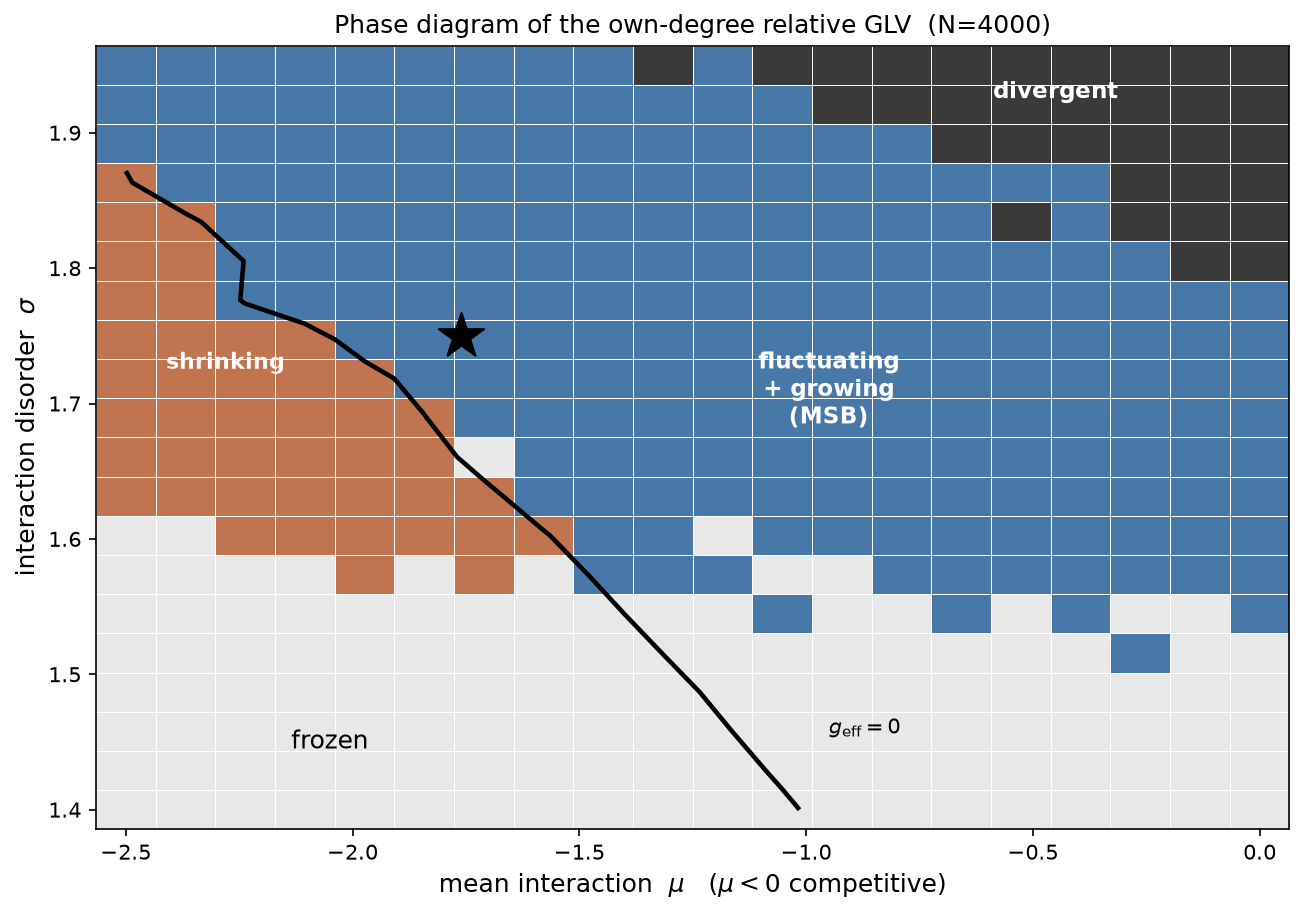
\includegraphics[width=\linewidth]{phase_diagram.png}
    \caption{Phase diagram of the relative model \eqref{eq:relative-glv} under the
    own-degree normalization, over the mean interaction $\mu$ (competitive for $\mu < 0$)
    and the disorder $\sigma$, classified from the late-time dynamics ($N = 4000$, a
    $20 \times 20$ grid with ten realizations per cell). At low disorder the shape relaxes and nothing fluctuates
    (frozen). Above it the dynamics are chaotic, and the solid black line marks the growth
    boundary $g_{\mathrm{eff}} = 0$, which separates the shrinking region ($g_{\mathrm{eff}}
    < 0$) from the fluctuating, growing band in which the firm-growth statistics are
    measured (blue, labelled MSB). The band is bounded below by the freezing line, on the
    competitive side by $g_{\mathrm{eff}} = 0$, and in the strong-disorder corner by the
    explosive, divergent region. The star marks the operating point $\mu = -1.76$,
    $\sigma = 1.75$. The band is an extended region, not a single point.}
    \label{fig:phase-diagram}
\end{figure}

This phase structure is not merely observed but can be derived. The relative model
\eqref{eq:relative-glv} is a disordered replicator equation, and its dynamical mean-field theory,
worked out in Appendix~\ref{app:dmft}, reduces the $N$-firm dynamics to a single representative
firm in a self-consistent Gaussian field. On a regular graph it gives the chaos onset in closed
form, $\sigma_c = \sqrt{2}$, independent of $\mu$. The mean interaction enters every firm's
fitness as the same uniform shift, so it cancels from the replicator and only sets the level of
the growth rate $g_{\mathrm{eff}}$, moving the $g_{\mathrm{eff}} = 0$ line but not the chaos
threshold. Below $\sigma_c$ the relaxed fixed point is the survivor law of the disordered
Lotka--Volterra model with the carrying capacity renormalized by the growth rate, and a direct
simulation on the matching ensemble confirms the predicted growth rate and surviving fraction to
about one percent, the fluctuations switching on exactly at $\sigma_c$. The fluctuating phase
itself, where the firm-growth statistics live, lies beyond this static fixed-point theory and
would need its two-time extension; we measure it directly instead.

Figure~\ref{fig:growing-churn} shows a single run in this regime. The total abundance (left)
climbs as a straight line in $\log M$ over the whole integration, the steady exponential growth
of \eqref{eq:Mdot-relative}, with no sign of a blow-up. The relative firm sizes $S_i = N y_i$
(right) do not settle; after an initial transient they keep exchanging rank and spanning orders
of magnitude, the persistent chaos of the $\sigma > \sigma_c$ phase. The economy grows while its
composition keeps turning over.

\begin{figure}[htbp]
    \centering
    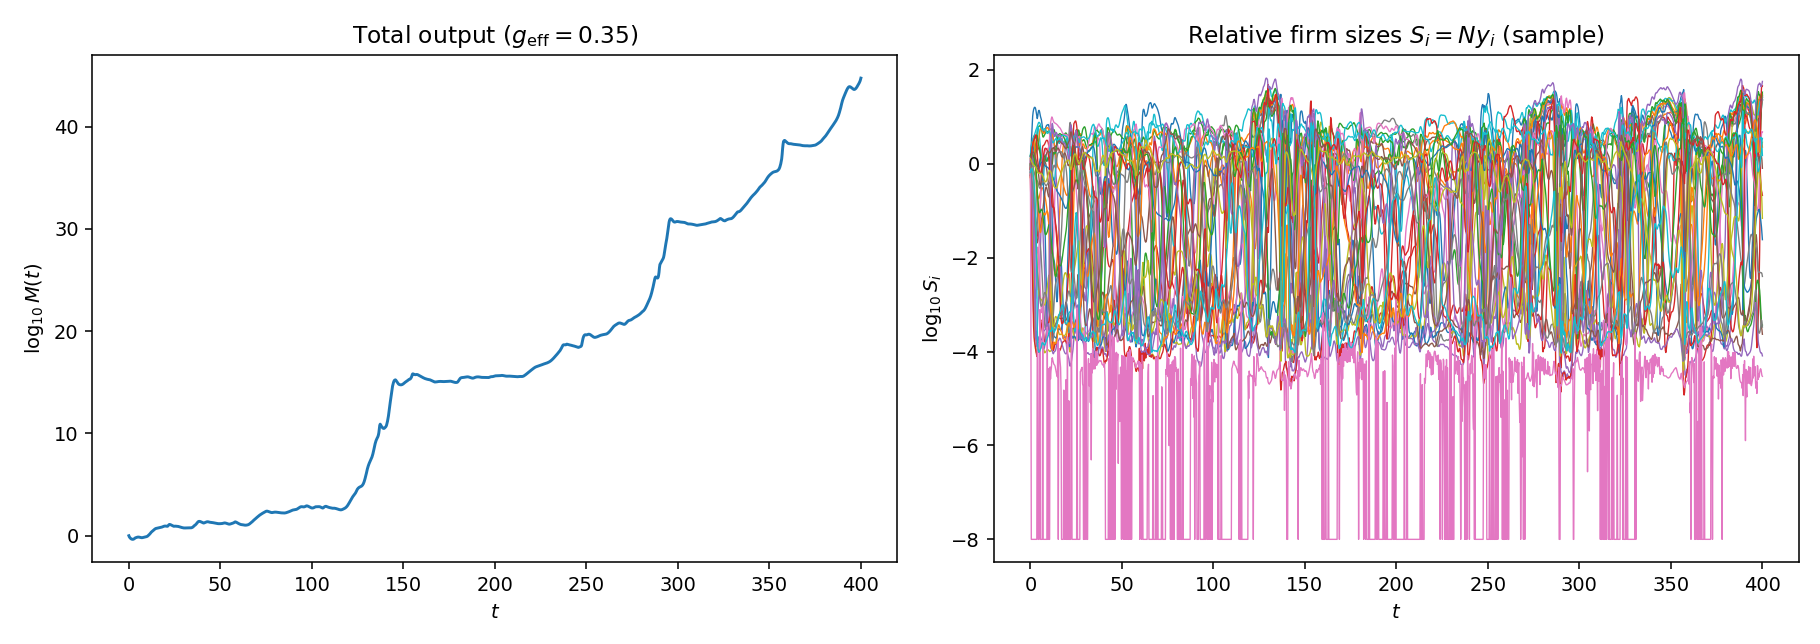
\includegraphics[width=\linewidth]{growing_growth_churn.png}
    \caption{A single run of the relative model \eqref{eq:relative-glv} at $\mu = -1.76$,
    $\sigma = 1.75$, $\lambda = 10^{-3}$ on a power-law graph with $N = 3000$. \panel{Left}: the
    total abundance grows exponentially in physical time, $\log_{10} M(t)$ rising
    linearly, with no finite-time divergence. \panel{Right}: a sample of relative firm sizes
    $S_i = N y_i$, which keep fluctuating and exchanging rank rather than relaxing to a
    fixed point.}
    \label{fig:growing-churn}
\end{figure}

\chapter{Firm-growth statistics}
\label{chap:firmgrowth}

\section{Firm-growth statistics in the fluctuating state}
\label{sec:growing-observables}

We measure the two firm-growth facts on the relative sizes $S_i = N y_i$, whose
cross-sectional mean is one by construction. The common growth of the economy is divided
out in the same step, since $\ln S_i = \ln x_i - \ln M + \ln N$, so the size and its
growth $g_i = \Delta \ln S_i$ are the idiosyncratic part of a firm's trajectory, exactly
what the data measure. We follow the empirical protocol: each firm contributes while it
is listed, that is while $S_i$ stays above the immigration floor, and we read growth
rates over a fixed yearly horizon $\Delta t$ rather than the solver's adaptive one. All
statistics are taken in a late window, after the initial relaxation has passed, and
restricted to firms that persist across it.

Two cautions, detailed in Appendix~\ref{app:numerics}, shape the measurement: the
per-firm volatility is a mean-absolute-deviation estimator robust to the fat tails, and
the size--volatility relation is fitted only over its power-law range, the decline above
the small-firm plateau set by the immigration floor.

Figure~\ref{fig:growing-msb} shows both observables at the operating point
$\mu = -1.76$, $\sigma = 1.75$ marked in Figure~\ref{fig:phase-diagram}, in the
stationary fluctuating state. The size--volatility relation (left) now falls
monotonically over the fitted range, $\sigma(\bar S) \sim \bar S^{-\beta}$ with a clean
power law ($R^2 \approx 0.98$ in the economy shown), in contrast to the rising V of
Appendix~\ref{chap:results}: large firms are now less volatile than small ones, as in the
data. The growth-rate distribution (right) is
sharply peaked and fat-tailed, with both flanks heavier than the Laplace reference and
no systematic asymmetry between them. The two facts that the static critical model could
not deliver together, a monotone size--volatility decay and a symmetric fat-tailed tent,
are both present here, and both are stationary properties of the chaotic state rather
than transients of a relaxation.

\begin{figure}[htbp]
    \centering
    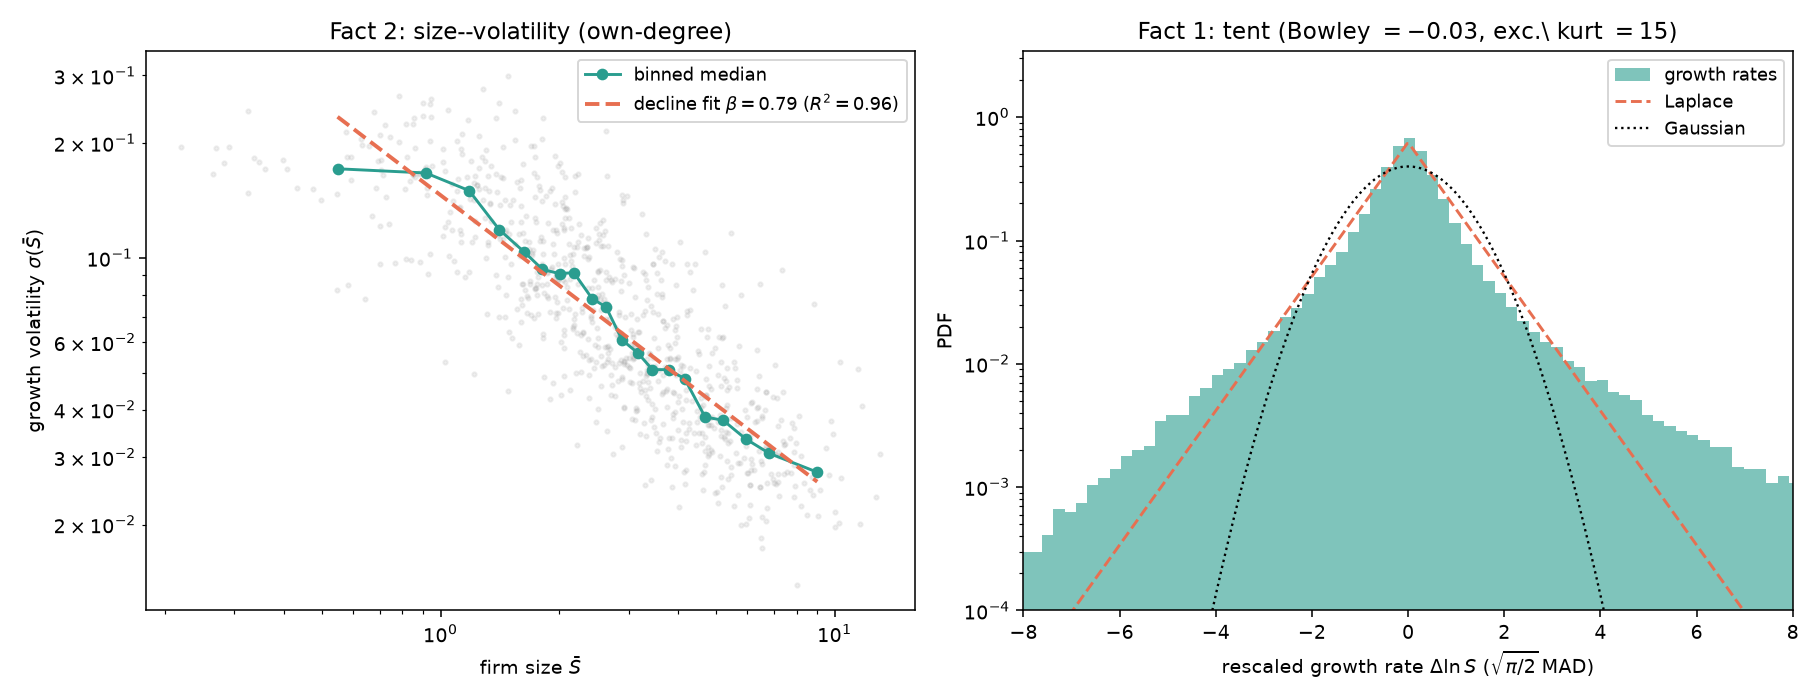
\includegraphics[width=\linewidth]{growing_stationary_msb.png}
    \caption{Firm-growth statistics at $\mu = -1.76$, $\sigma = 1.75$. Left: the
    size--volatility relation in a single economy ($N = 6400$) under the global mean-degree
    normalization; volatility falls as a
    power law over the fitted decline above the small-firm immigration-floor plateau
    (shaded), here with exponent $\beta \approx 0.5$ and $R^2 = 0.98$. Right: the
    growth-rate distribution pooled over economies, sharply peaked and fat-tailed,
    heavier than the Laplace reference on both flanks and close to symmetric
    (Bowley $\approx 0$), far above the Gaussian.}
    \label{fig:growing-msb}
\end{figure}

\section{Finite size and the mean-field limit}
\label{sec:growing-finite-size}

The chaotic state above is not equally robust at all system sizes, and the way it
strengthens with $N$ both validates the measurement and bears on the
size--variance exponent, which depends on the size of the economy rather than approaching
a fixed value. At small $N$ the persistent chaos is fragile: for many graph
realizations the shape, after fluctuating for a while, eventually collapses onto a fixed
point and freezes, recovering the relaxation transient of Appendix~\ref{chap:results}.
This is the known finite-size metastability of the fluctuating phase
\citep{roy2020}: rare large excursions drive firms below the floor, and the state can
fall into a frozen attractor. Figure~\ref{fig:growing-trajectories} contrasts the two
outcomes directly, a realization that freezes onto a fixed point against one that keeps
churning to the end of the run. Measuring in a short early window, as one is
tempted to do, reports the firms while they still fluctuate and so mistakes the frozen
transient for a stationary state; only integrating to long times separates the two.

\begin{figure}[htbp]
    \centering
    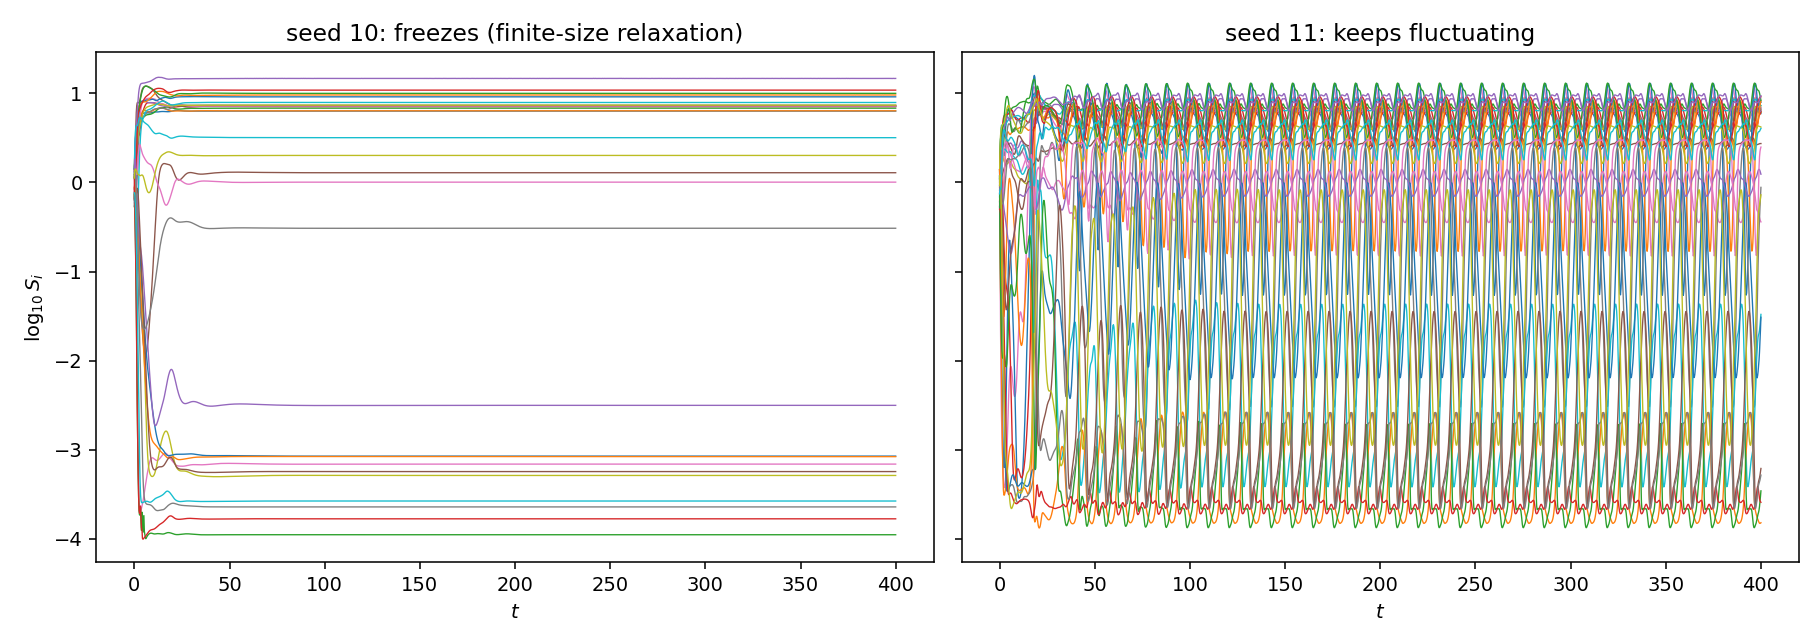
\includegraphics[width=\linewidth]{growing_trajectories.png}
    \caption{Two finite-size realizations at $N = 600$, $\mu = -1.76$, $\sigma = 1.75$.
    Left: the shares churn for a while and then freeze onto a fixed point, the
    finite-size relaxation transient. Right: a realization in which the chaos persists
    for the whole run. Whether a given realization freezes or keeps fluctuating is a
    finite-size accident that becomes rarer as $N$ grows.}
    \label{fig:growing-trajectories}
\end{figure}

Whether a realization freezes or keeps fluctuating is a finite-size accident that
becomes rarer as $N$ grows. The left panel of Figure~\ref{fig:growing-meanfield}
records the fraction of realizations that remain persistently chaotic at long times: it
is fragile at small $N$, with half to three-quarters of realizations persisting, and
reaches all of them by $N \approx 6000$. The fragility is
a finite-size effect; in the mean-field limit the fluctuating phase is the generic
outcome of the operating regime, consistent with the dynamical mean-field picture of
\citet{bunin2017} and \citet{roy2020}.

The size--variance exponent is a subtler matter, and turns on how the competition is
shared across the heterogeneous graph; its magnitude is the shallower of the two
comparisons we can make with the data. Under the global mean-degree normalization the exponent is not fixed by the mean-field limit:
measured on the persistent realizations it falls steadily and monotonically with system
size, from about $0.68$ at $N = 800$ toward $0.25$ at $N = 1.3\times10^4$
(Fig.~\ref{fig:growing-meanfield}, right), and it does not approach a nonzero constant.
There is no thermodynamic plateau to read off: an earlier fit of
$\beta(N) = \beta_\infty + c\,N^{-1/2}$ to an apparent intercept inside the band forced a
finite limit on a quantity that keeps falling, and rested in addition on a survivor
criterion that biases the measurement.

The exponent must instead be read at a finite economy size, because the data are, and on
the firm set the data actually use. We follow the empirical protocol: a firm is listed
while its size exceeds a fixed fraction of the mean firm and contributes growth rates only
while listed, keeping those with at least twenty such rates, as in the sample of
$15{,}788$ listed firms of \citet{moran2024}. Coexistence is then extensive, the
participation ratio $D_{\mathrm{eff}} = 1/\sum_i \bar w_i^2$ growing in proportion to $N$
and between $65$ and $78$ per cent of firms active at any time, in line with the $65$ per
cent of the empirical panel that enters the volatility estimate. The exponent on this
active set falls in the same way, and at the economy size for which the number of active
firms equals that sample, $N \approx 2\times10^4$, it is $\beta \approx 0.15$, at the
lower edge of the empirical band $0.15$--$0.20$ (Fig.~\ref{fig:growing-finite-economy}).
We read this as a finite-economy-size
effect rather than a thermodynamic exponent: real listed economies are finite, of order
$10^4$ firms, and the model reproduces the empirical exponent at that scale while
predicting a smaller one for a larger listed universe. The earlier impression of a
plateau inside the band, and the opposite worry of a collapse toward zero, were two faces
of one survivor artifact, since holding the delisting threshold fixed in share units while
the mean share falls as $1/N$ drops a growing fraction of firms through single transient
excursions; with delisting defined relative to the mean firm, as in the data, the active
population is extensive and the exponent sits at the empirical scale in the empirical
range.

\begin{figure}[htbp]
    \centering
    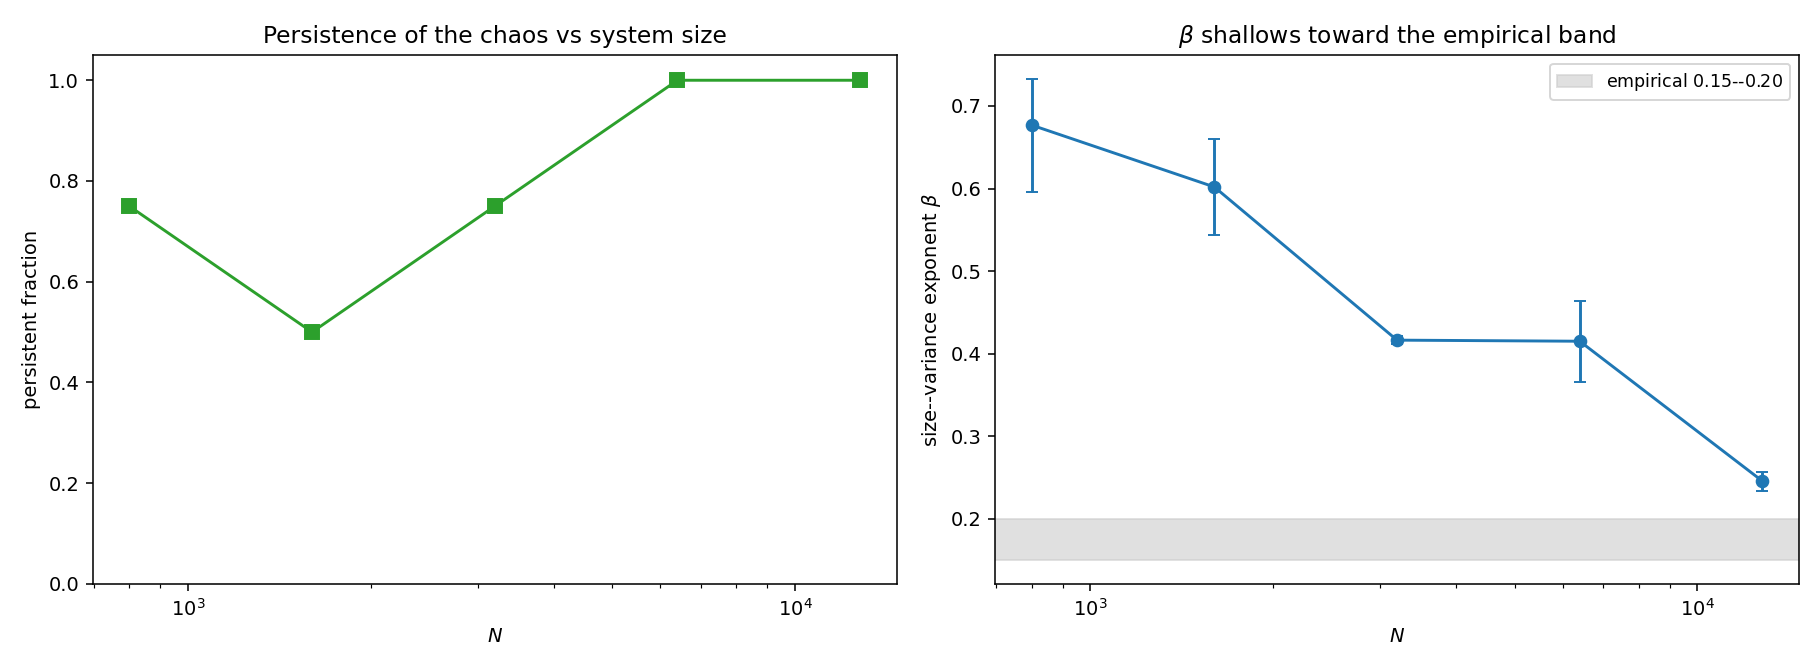
\includegraphics[width=\linewidth]{growing_meanfield.png}
    \caption{Approach to the mean-field limit at $\mu = -1.76$, $\sigma = 1.75$,
    $\lambda = 10^{-3}$. Left: the fraction of realizations that stay persistently
    chaotic at long times rises to one by $N \approx 6000$, so the finite-size
    fragility of the fluctuating phase is a finite-$N$ effect. Right: the
    size--variance exponent $\beta$ measured on the surviving firms falls steadily as $N$
    grows, through the empirical band (shaded); its value at a finite economy size is read
    with the empirical listed-firm protocol in the text.}
    \label{fig:growing-meanfield}
\end{figure}

\begin{figure}[htbp]
    \centering
    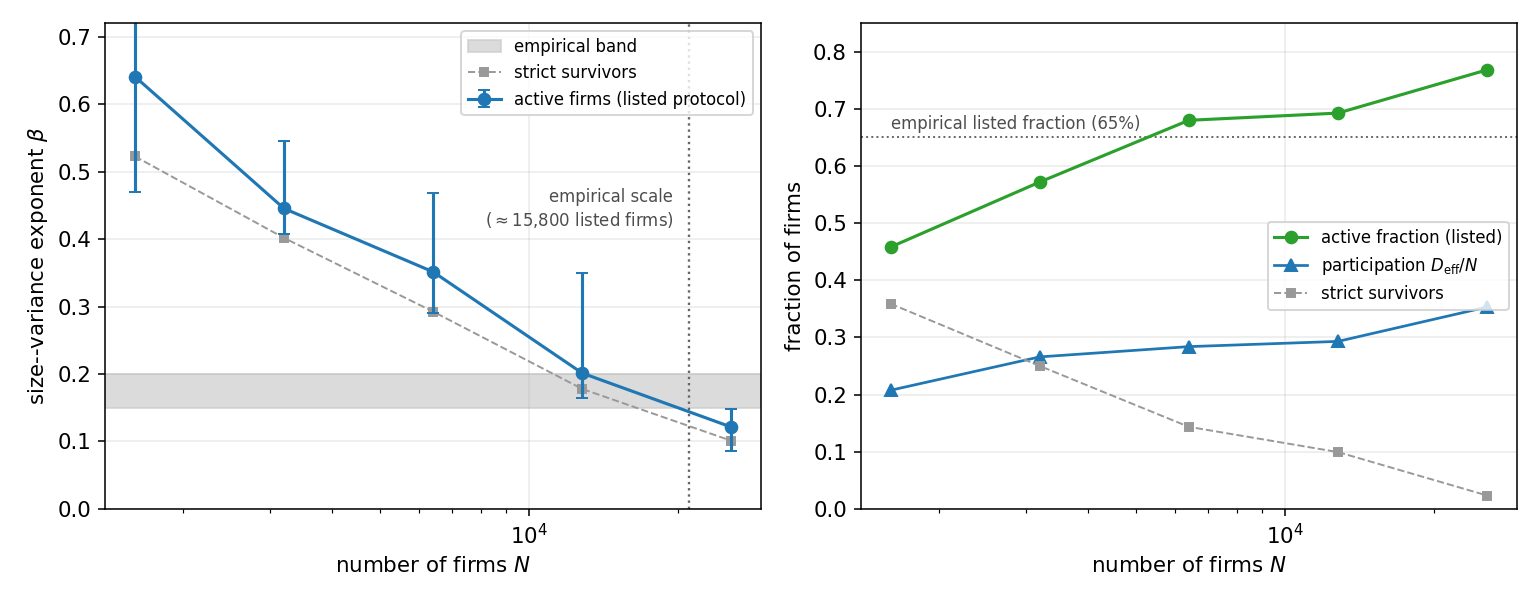
\includegraphics[width=\linewidth]{growing_finite_economy.png}
    \caption{The size--variance exponent and coexistence under the empirical listed-firm
    protocol, at $\mu = -1.76$, $\sigma = 1.75$, $\lambda = 10^{-3}$. A firm is counted
    while its relative size exceeds one per cent of the mean firm and contributes growth
    rates only then, retaining firms with at least twenty rates. Left: the exponent
    $\beta$ falls through the empirical band (shaded) as the economy grows; the dotted line
    marks the economy size at which the number of active firms equals the empirical sample
    of about $15{,}800$ listed firms, where $\beta \approx 0.15$, at the lower edge of the
    band. The strict never-delisted survivors (dashed) give a slightly lower exponent, the
    calm-subsample selection bias. Right: coexistence is extensive, the active fraction and
    the participation ratio $D_{\mathrm{eff}}/N$ both roughly flat in $N$ and near the
    empirical listed fraction, while the strict survivor count (dashed) falls only because
    its fixed share floor becomes a stiffer cutoff as the mean share shrinks. Error bars
    are the interquartile spread over graph realizations.}
    \label{fig:growing-finite-economy}
\end{figure}

Under the own-degree normalization each firm's couplings are scaled by its own degree, so
that every firm carries a disorder field of the same variance whatever its connectivity,
the natural per-fan-in scaling on a heterogeneous graph. The exponent is then a clean
power law that is robust across system size, a genuine thermodynamic quantity, but its
value is steeper, $\beta \approx 0.7$, about three times the empirical one. The two normalizations therefore trade against each other on
magnitude: the mean-degree one reaches the empirical value at the empirical economy size,
the own-degree one fixes a size-independent exponent that is too steep. The difference is
the hubs, which the mean-degree normalization over-couples, a node accumulating a disorder
field that grows with its degree, and which the own-degree normalization quiets to a
common one. Magnitude, however, is not where the granular models fail.

\section{Higher moments and the multiscaling}
\label{sec:growing-multiscaling}

The size--variance exponent is only the first moment of a richer object, the distribution
of growth volatility conditional on size, and it is on the higher moments that the
granular models break. \citet{moran2024} show that the $q$-th moment of the
size-conditioned volatility decays as a power law, $E[\sigma^q \mid S] \sim S^{-\zeta_q}$,
but with an exponent that depends on the order $q$: in the data
$\zeta_1,\dots,\zeta_4 \approx 0.20,\,0.39,\,0.51,\,0.58$, rising with $q$. A granular
composition of independent sub-units predicts the opposite, an exponent independent of
$q$, so this multiscaling is the observable the granular picture cannot reproduce, and the
one \citet{moran2024} read as the fingerprint of correlations that grow with firm size.

The own-degree relative GLV reproduces it. Figure~\ref{fig:growing-multiscaling} measures
the first four moments of the size-conditioned volatility in the model and fits each on
its decline branch. The exponents rise with the order,
$\zeta_1,\dots,\zeta_4 \approx 0.67,\,1.26,\,1.73,\,2.06$; their overall scale is the
steep one of the own-degree normalization, but once divided by $\zeta_1$ the
$q$-dependence, $1,\,1.9,\,2.6,\,3.1$, lies almost on top of the empirical
$1,\,2.0,\,2.6,\,2.9$ and far from the flat granular prediction (right panel). The model
produces the same anomalous scaling of the higher moments as the data, with no internal
firm structure and nothing put in by hand: the size-growing correlations the granular
picture must assume are generated here by the interactions.

The mean-degree normalization fails this test, and instructively. Its over-coupled hubs
give the largest firms a heavy-tailed volatility, so the higher moments are dominated by a
volatile minority and rise with size rather than falling; the measured $\zeta_q$ decrease
with $q$ and turn negative by $q = 4$, the opposite of the data. The discriminating
observable thus picks out the own-degree normalization, the one that quiets the hubs into
the thin-tailed volatility distribution the data show.

\begin{figure}[htbp]
    \centering
    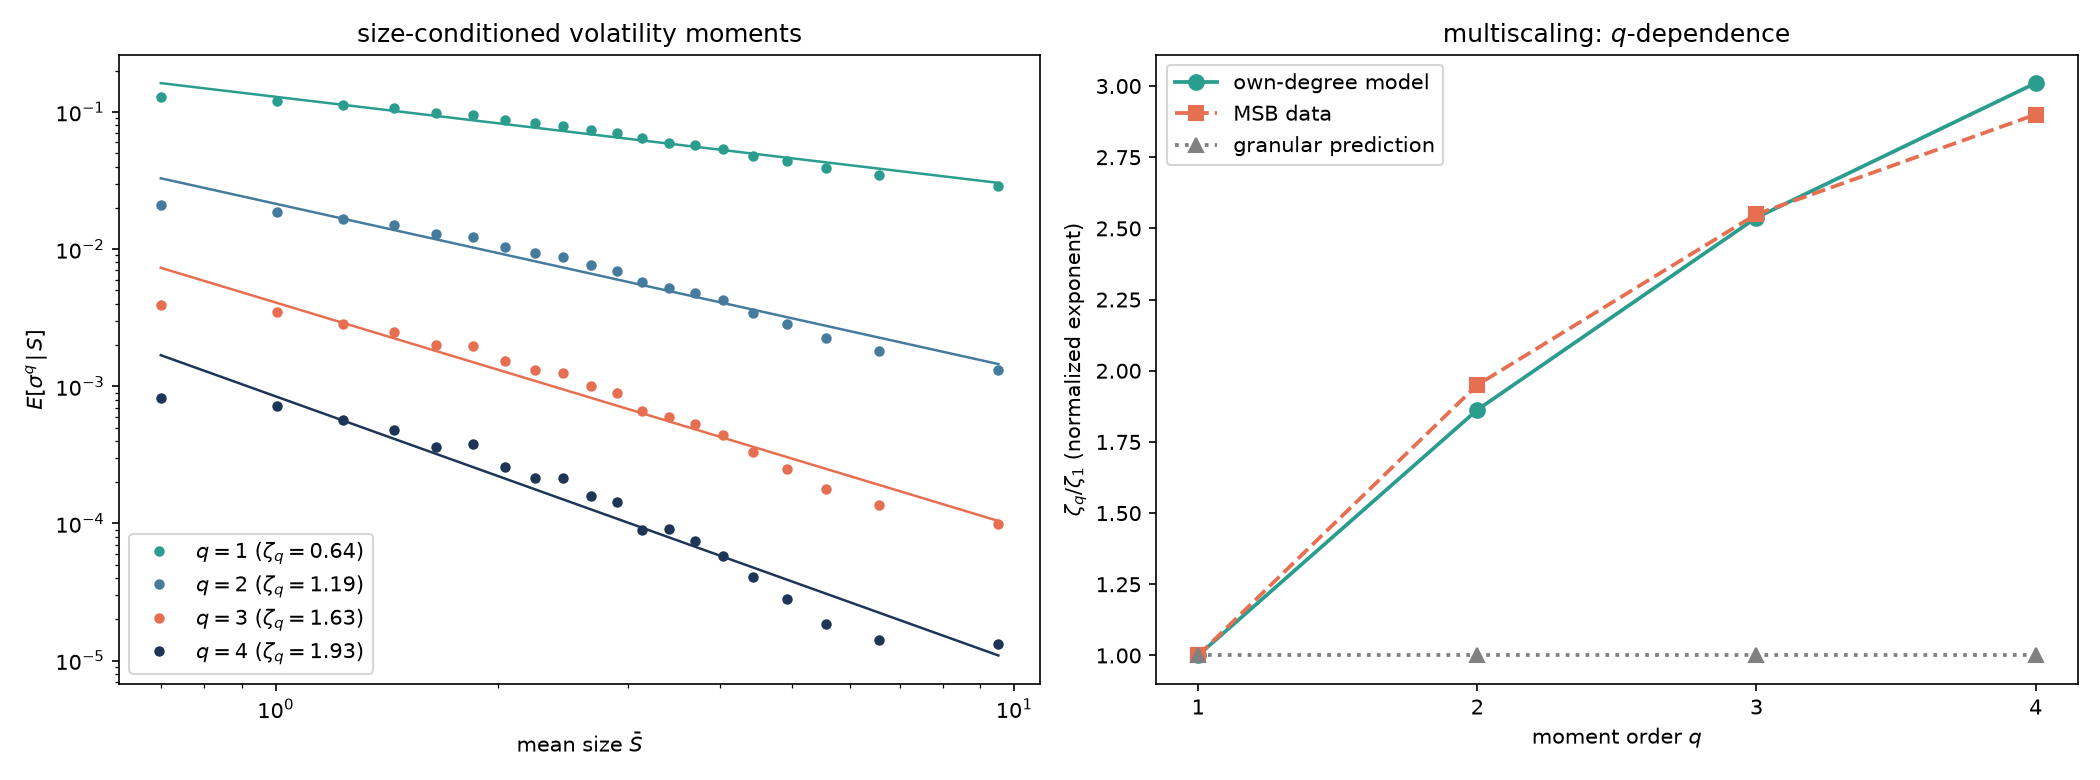
\includegraphics[width=\linewidth]{growing_multiscaling.png}
    \caption{Multiscaling of the size-conditioned volatility in the own-degree model,
    $\mu = -1.76$, $\sigma = 1.75$. Left: the first four moments $E[\sigma^q \mid S]$
    against mean size on a double-logarithmic scale, each fitted on its decline branch;
    the slopes steepen with the order $q$, giving exponents
    $\zeta_1,\dots,\zeta_4 \approx 0.67,\,1.26,\,1.73,\,2.06$. Right: the exponents
    normalized by the first, $\zeta_q/\zeta_1$, against the moment order, for the model,
    the data of \citet{moran2024}, and the granular prediction of a $q$-independent
    exponent. The model reproduces the empirical $q$-dependence and refutes the granular
    one; only the overall scale differs, the own-degree exponent being about three times
    the empirical.}
    \label{fig:growing-multiscaling}
\end{figure}

The multiscaling is one of three size-conditioned tests by which \citet{moran2024}
separate the data from the granular models, and the own-degree relative GLV passes the
other two as well (Fig.~\ref{fig:growing-conditional}). The first is a collapse: rescaled
by its size-conditional mean, the per-firm volatility distribution $\sigma_i/\bar\sigma(S)$
is the same at every size, with a bounded tail, as in the data. The second is the sharper.
Were a firm an aggregate of many independent parts, the central limit theorem would drive
its growth distribution toward a Gaussian as it grew, the excess kurtosis falling to zero
with size; the data do the opposite, large firms remaining at least as fat-tailed as small
ones. The model reproduces this anti-Gaussian trend, the excess kurtosis of the
size-unmixed growth rising from about three for the smallest firms to ten for the largest,
the signature that a firm's growth is not a sum of independent contributions but carries
the correlations the interactions impose. The model thus clears not only the
size--variance exponent that the granular models also fit, but every conditional test by
which the data reject them.

\begin{figure}[htbp]
    \centering
    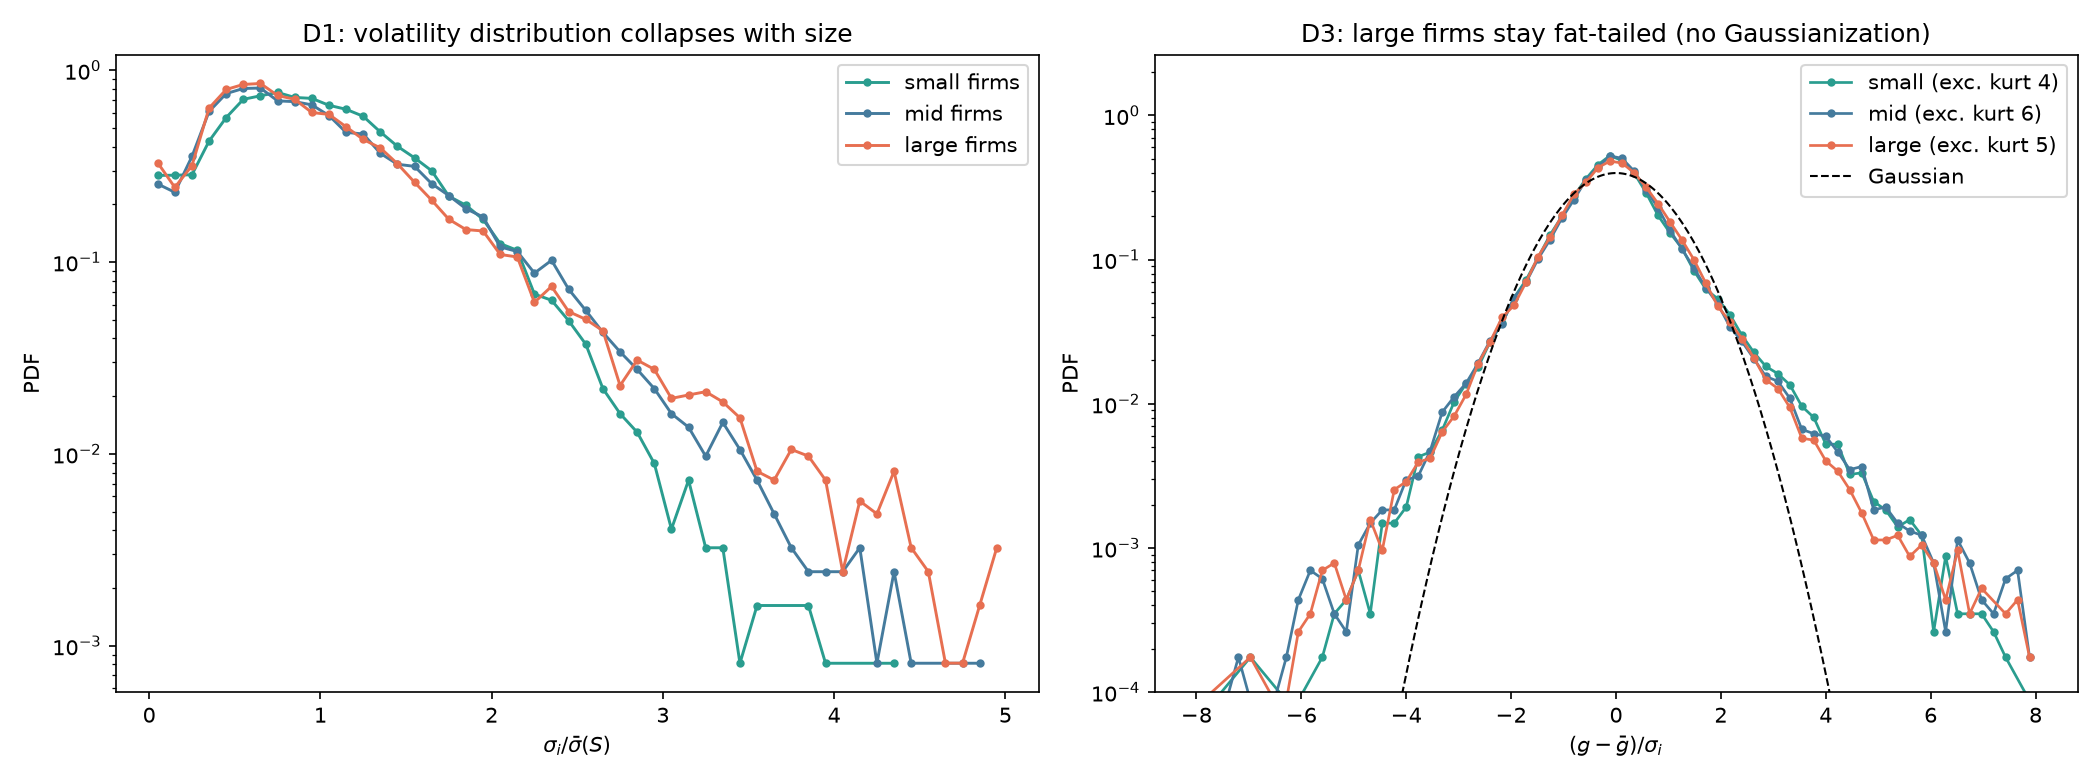
\includegraphics[width=\linewidth]{growing_conditional.png}
    \caption{The other two discriminating tests of \citet{moran2024}, on the own-degree
    model. Left (D1): the per-firm volatility distribution, rescaled by its
    size-conditional mean $\sigma_i/\bar\sigma(S)$, collapses onto a single size-independent
    shape with a bounded tail. Right (D3): the size-unmixed growth $(g-\bar g)/\sigma_i$
    stays fat-tailed at every size, well above the Gaussian, and the largest firms are the
    fattest, the excess kurtosis rising from about three to ten with size, rather than
    approaching a Gaussian as an aggregate of independent parts would.}
    \label{fig:growing-conditional}
\end{figure}

The dependence on the normalization is itself informative, and it shows that the gap in
magnitude cannot be closed within this family without losing the structure. Writing the
noise scaling as $\sigma/k_i^{\,p}$, with $p = 0$ the mean-degree normalization and
$p = \tfrac12$ the own-degree one, sweeps the hub loudness continuously, and with it both
the exponent and its higher moments (Fig.~\ref{fig:growing-normalization}). The
first-moment exponent rises monotonically with $p$, from about $0.15$ at $p = 0$ to $0.69$
at $p = \tfrac12$, and reaches the empirical band only at $p = 0$. The multiscaling matches
the data only at the other end, $p \gtrsim 0.4$, where $\beta$ is two to three times too
steep; as $p$ falls and $\beta$ comes down the higher-moment exponents flatten, and by
$p = 0$ they invert, the moments rising with size rather than falling. The two never
coincide. The hub-quieting that produces the thin-tailed multiscaling is the same that
over-stabilizes the largest firms, so bringing $\beta$ into the band requires loud hubs,
which destroy the structure. Magnitude and multiscaling are two faces of one parameter,
and no normalization in this family yields both at once. The gap is therefore not a matter
of calibration but of a missing ingredient, the size-dependent correlations of a firm
built from many parts, which the single-level model cannot supply.

\begin{figure}[htbp]
    \centering
    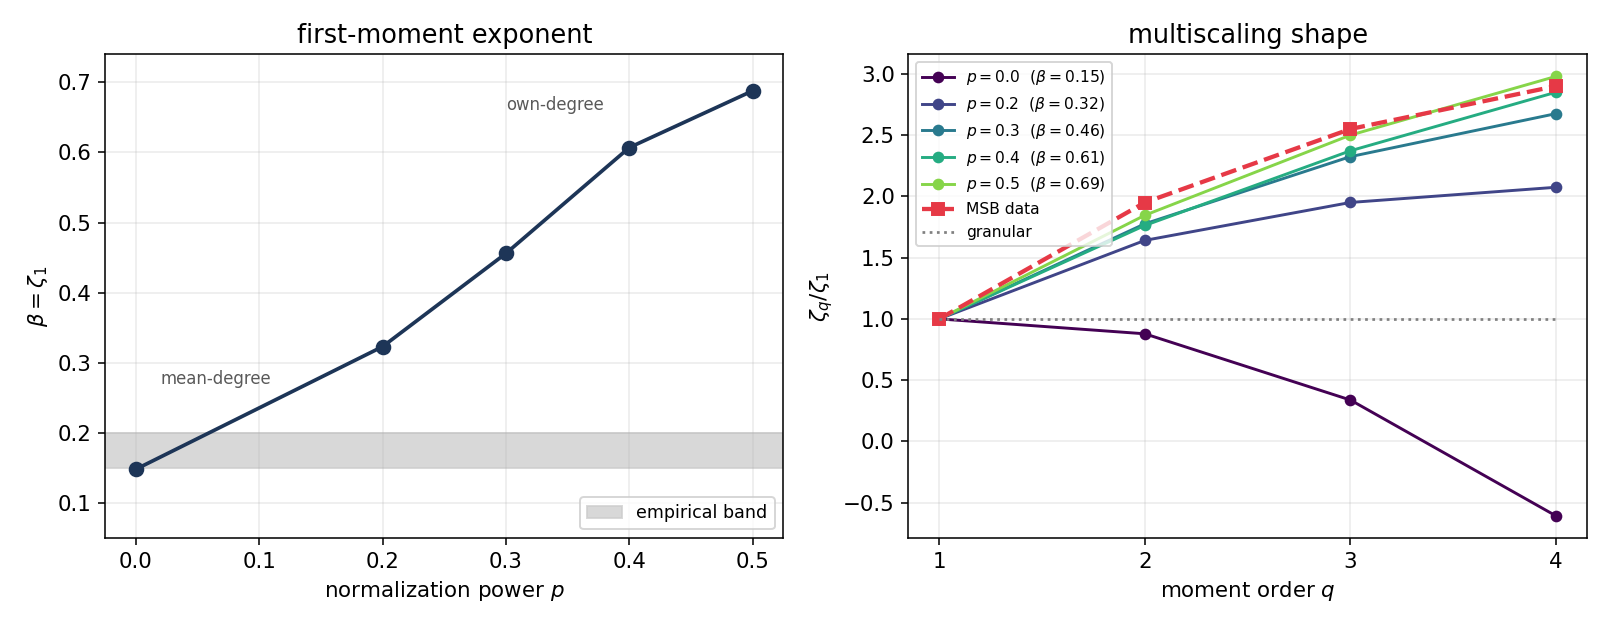
\includegraphics[width=\linewidth]{growing_normalization.png}
    \caption{The magnitude--structure trade-off across the normalization family, the noise
    scaled as $\sigma/k_i^{\,p}$, at $\mu = -1.76$, $\sigma = 1.75$, $N = 1.3\times10^4$;
    $p = 0$ is the mean-degree normalization and $p = \tfrac12$ the own-degree one. Left:
    the first-moment exponent $\beta = \zeta_1$ rises monotonically with $p$ and enters the
    empirical band (shaded) only at $p = 0$. Right: the normalized higher-moment exponents
    $\zeta_q/\zeta_1$ match the data of \citet{moran2024} only for $p \gtrsim 0.4$, where
    $\beta$ is far too steep, and collapse, inverting by the fourth moment, at the $p = 0$
    where $\beta$ lies in the band. No single $p$ reproduces both the magnitude and the
    multiscaling.}
    \label{fig:growing-normalization}
\end{figure}

\section{The role of the interactions}
\label{sec:growing-ablation}

The model carries no external heterogeneity and no explicit noise: the only source of
fluctuation is the disordered interaction matrix. To confirm that the firm-growth
statistics are produced by the interactions, and are not an artifact of the
multiplicative structure or the immigration floor, we switch the disorder off and dial
it back up. Table~\ref{tab:growing-ablation} sweeps $\sigma$ at fixed $\mu$, $\lambda$
and $N$. Below the threshold $\sigma_c = \sqrt{2}$ the dynamics freeze: the late-time
growth fluctuations are zero to the precision quoted, the shape has relaxed to a fixed
point, and there is no fluctuating state to measure. The persistent fluctuations and
the fat-tailed tent appear only once $\sigma$ crosses $\sigma_c$, growing with the
disorder. With no noise in the model, the fluctuations can come only from the disorder,
and removing it removes them entirely.

\begin{table}[h]
    \centering
    \begin{tabular}{rccc}
        \hline
        $\sigma$ & growth fluctuation & excess kurtosis & fat-tailed tent? \\
        \hline
        $0.00$ & $0.000$ & --   & no  \\
        $0.50$ & $0.000$ & --   & no  \\
        $1.00$ & $0.000$ & --   & no  \\
        $1.41$ & $0.000$ & --   & no  \\
        $1.60$ & $0.085$ & $14$ & yes \\
        $1.75$ & $0.175$ & $14$ & yes \\
        \hline
    \end{tabular}
    \caption{Disorder ablation at $\mu = -1.76$, $\lambda = 10^{-3}$, $N = 3200$ on a
    power-law graph. ``Growth fluctuation'' is the standard deviation of the pooled
    late-window growth rates. Below the chaotic threshold $\sigma_c = \sqrt{2}$ the state
    freezes (growth fluctuation zero to the precision quoted) and there is no genuine
    fluctuating distribution to characterize, so the kurtosis is left blank; the
    persistent fluctuations and the fat-tailed tent switch on only once $\sigma$ crosses
    $\sigma_c$. (A nonzero $\beta$ can still be fitted below threshold, but on a frozen
    state during its relaxation, the V transient of Appendix~\ref{chap:results}, not on a
    stationary fluctuating law.)}
    \label{tab:growing-ablation}
\end{table}

This is the distinction the introduction asked for. The firm-growth statistics here are
a between-firm effect, generated by the network of interactions, and not a within-firm
one: with the interactions removed there is nothing left, no noise carrying the
fluctuations and no single-firm mechanism producing a tail. It is also the size of the
result that separates this model from the simplest alternatives. A growing economy with
a stationary heavy-tailed size distribution can be had from a mean-field multiplicative
model with injected noise \citep{bouchaudmezard2000}, but there the fluctuations are put
in by hand and there is no network. Here the same growing aggregate, the heavy tails,
and the slow size--variance decay arise together from a single ingredient, the disordered
interactions, which is the size-dependent correlation mechanism \citet{moran2024}
identify as the one the granular models lack.

\section{Discussion}
\label{sec:growing-discussion}

This chapter closes the gap left by Appendix~\ref{chap:results}. Making the
Lotka--Volterra interactions relative to the mean firm turns the finite-time divergence
of the standard model into steady exponential growth, and in the disordered regime
$\sigma > \sigma_c$ the resulting economy grows while its composition fluctuates without
ever settling. In this genuinely nonstationary state the size--variance relation is a
stationary law that falls with the empirical sign; it clears the conditional tests by
which the data reject the granular models, the anomalous multiscaling of its higher
moments and the persistence of fat tails in the largest firms; the growth-rate
distribution is symmetric and fat-tailed; and switching off the disorder removes them all,
placing their origin in the interactions.

Three honest qualifications bound the claim. The model itself is not new: it is the
disordered replicator equation \citep{diederich1989,hofbauer81}, equivalently the
chaotic phase of the disordered Lotka--Volterra model \citep{bunin2017,galla2018,roy2020},
and its finite-size fragility and approach to a robust mean-field fluctuating phase are
known features of that system. What is specific here is the use of this state, on a
heterogeneous graph and with the interactions made relative so that the aggregate grows,
as a model of firm growth, and the finding that its firm-growth statistics match the
empirical ones. The exponent's magnitude, second, is matched only up to the
normalization of the couplings: with the own-degree scaling it is a clean thermodynamic
power law but about three times too steep, while with the mean-degree scaling it reaches
the empirical value at the observed economy size of order $10^4$ listed firms but does not
settle to a thermodynamic constant. It is the order-dependence of the higher moments, not
the magnitude of the first, that the model reproduces and the granular picture does not.
Third, the economy grows in the large
majority of realizations rather than in every one, the operating point sitting in the
growing band but not far from its $g_{\mathrm{eff}} = 0$ boundary. Beyond these, what the model adds that the granular picture cannot is the multiscaling of
the higher moments, the signature \citet{moran2024} read as correlations that grow with
firm size; measuring that correlation structure directly,
rather than through its moments, and closing the factor of three in the exponent's
magnitude, which we have shown no normalization in this family can do, are the natural
next steps, both pointing to the same missing ingredient, a firm built from many
correlated parts.

\chapter{Conclusion}
\label{chap:conclusion}

This thesis asked whether a dynamical model of interacting firms can generate the two
firm-growth anomalies on its own, without the heavy-tailed internal composition that the
granular models assume and that \citet{moran2024} show the data reject. The answer it
reaches is that it can. Working with a Generalized Lotka--Volterra network and nothing
else, no externally imposed heterogeneity, no injected noise, and no built-in
correlations, we recover both the fat-tailed growth-rate distribution and a
size--variance relation that falls with the empirical sign, as stationary properties of
a persistently fluctuating economy that grows.

The model is a single change to the standard Generalized Lotka--Volterra system: the
self-limitation and the interactions act on a firm's size relative to the average firm
rather than on its absolute size. This makes the dynamics scale-invariant, so the total
output grows exponentially without the finite-time blow-up of the absolute model, while
in the strongly disordered regime the composition of the economy never settles but keeps
churning chaotically. In that state the two facts hold together and prove robust,
surviving as the graph, the system size, and the sampling interval are varied, and
switching off the disorder removes them entirely, which places their origin
in the interactions themselves rather than in any property of a single firm. The change
was forced by what the absolute model cannot do: tuned to its cooperative critical point
it reproduces the heavy tails but its size--variance relation is only a relaxation
transient, the trace of an arbitrary initial condition settling onto the critical
attractor rather than a stationary law, so that recovering a genuine law calls for a
state that keeps fluctuating instead of relaxing. That analysis, and the coordinate
change and time rescaling that make the critical point reachable at all, are collected in
the appendices.

What the thesis contributes is a model, not a mechanism read off from the data. The
granular and sub-unit pictures posit the source of the fluctuations, a fixed heavy-tailed
composition of parts within each firm; the mean-field multiplicative models that also
produce a growing economy with heavy tails put the noise in by hand and carry no network
\citep{bouchaudmezard2000}. Here the same phenomenology, the heavy tails, the slow
size--variance decay, the growing aggregate, and the perpetual turnover of firms, follows
from a single deterministic ingredient, the disordered couplings between companies. The
size-dependent correlations that \citet{moran2024} identify as the missing element are
then not assumed but produced, and the model turns them from a hypothesis one must accept
into something one can measure. The shift is from a within-firm account, in which a
company's volatility is fixed by how its own activities are composed, to a between-firm
one, in which it emerges from the company's place in a fluctuating web of competitors,
which is the more natural home for the shared customers and suppliers the correlations
were attributed to in the first place.

Three qualifications bound the claim. The dynamics themselves are not new: the
fluctuating regime is the chaotic phase of the disordered Lotka--Volterra model,
equivalently the disordered replicator equation
\citep{diederich1989,bunin2017,galla2018,roy2020}, whose finite-size fragility and
approach to a robust mean-field fluctuating phase are already studied. What is specific
here is the construction that turns that state into a growing economy, the relative
interactions, and its use as a model of firm growth. The quantitative match, second, is
partial, and partial in an informative way: the model reproduces the order-dependent
multiscaling of the higher moments, the signature of size-growing correlations that the
granular models cannot produce, but the magnitude of the size--variance exponent is
matched only in sign. The exponent is a clean, size-independent power law, about four times
too steep, $\beta \approx 0.8$ against the empirical $0.15$--$0.20$. The same per-firm
scaling that quiets the disorder field into the correctly multiscaling volatility
distribution is what over-stabilizes the most connected firms and steepens the exponent, so the
steep magnitude and the correct multiscaling come out of the same per-firm scaling and cannot be
tuned apart, which points past the single-level model. Third, the growth is
near-critical: the operating
point that best reproduces the facts sits close to the boundary between a growing and a
shrinking economy, so the economy grows in most graph realizations but not in all of them.
None of these undoes the qualitative result, but each marks the distance between it and a
quantitative theory.

The natural next steps follow from these limits. Pinning the exponent and the
near-critical character of the growth would need many more realizations at the largest
system sizes, where the present estimates are noisiest. More fundamental is the
correlation structure itself: the match shown here is in the marginal facts and their
moments, the shape of the growth distribution and the scaling of its volatility, whereas
the size-dependent correlations \citet{moran2024} call for are something the model
generates directly and could be measured directly, firm by firm, rather than only through
their consequences. Doing so, and closing the gap in the magnitude of the exponent, both
point to the ingredient the single-level model still lacks, a firm built from many
correlated parts. Beyond that, replacing the schematic disordered graph with couplings closer to the
real economy, input--output linkages, supply networks, and shared markets, would be the
step from a model that reproduces the stylized facts to one that speaks to the
macroeconomic dynamics behind them.


\vspace{100pt}

\printbibliography

\appendix
\chapter{Dynamical mean-field theory of the relative model}
\label{app:dmft}
\providecommand{\Dz}{\mathcal{D}z}
\providecommand{\E}{\mathbb{E}}

This note derives a dynamical mean-field theory (DMFT) for the scale-invariant model of
the growing-economy chapter, in which the interactions act on the average firm rather
than on absolute abundances. The model turns out to be a disordered replicator equation,
so its DMFT is the heterogeneous single-site process already used to locate $\mu_c$
\citep{aguirrelopez}, with two small additions that the scale invariance forces. The
reduction to a replicator and the resulting effective single-site process and its
self-consistency conditions are set out below.

\section{The model and its reduction to a replicator}
\label{sec:dmft-model}

We take the relative GLV in the competition convention used in the simulations,
\begin{equation}
    \dot x_i = x_i\left[\,1 - \frac{x_i}{m} - \frac{(\alpha x)_i}{m}\,\right],
    \qquad m = \frac1N\sum_j x_j = \frac MN ,
    \label{eq:dmft-glv}
\end{equation}
with couplings on a graph of mean degree $C$,
\begin{equation}
    \alpha_{ij} = A_{ij}\Big(-\frac{\mu}{C} + \frac{\sigma}{\sqrt C}\,z_{ij}\Big),\qquad
    z_{ij}\sim\mathcal N(0,1),\qquad \overline{z_{ij}z_{ji}} = \gamma,\qquad \alpha_{ii}=0 .
\end{equation}
Both the self-limitation $x_i/m$ and the interaction $(\alpha x)_i/m$ are divided by the
population mean $m$. The right-hand side of \eqref{eq:dmft-glv} is then homogeneous of
degree one in $x$, so the bracket $F_i := 1 - x_i/m - (\alpha x)_i/m$ depends on $x$ only
through ratios. The overall scale is a free direction that grows or decays exponentially
without the finite-time blow-up of the absolute model.

Introduce the relative abundances $y_i = x_i/m$, which satisfy $\langle y\rangle :=
\frac1N\sum_i y_i = 1$ by construction, and let $M = \sum_j x_j$ be the total. The
aggregate grows at the population-averaged fitness,
\begin{equation}
    g(t) := \frac{d\ln M}{dt}
          = \frac1M\sum_j \dot x_j = \sum_j \frac{x_j}{M}\,F_j
          = \frac1N\sum_j y_j F_j = \langle yF\rangle .
    \label{eq:dmft-g}
\end{equation}
Subtracting this common scale leaves a closed equation for the relative abundances,
\begin{equation}
    \dot y_i = y_i\big(F_i - g(t)\big),\qquad
    F_i = 1 - y_i - (\alpha y)_i,\qquad
    g(t) = \langle yF\rangle ,
    \label{eq:dmft-replicator}
\end{equation}
which is a replicator equation, the simplex projection of \eqref{eq:dmft-glv} in the sense
of Hofbauer's correspondence \citep{hofbauer81}. The aggregate is recovered from
$M(t) = M(0)\exp\!\int_0^t g$, and a positive stationary $g$ is a steadily growing
economy.

\paragraph{What the $-g(t)$ term is.}
The drift $-g(t)$ in \eqref{eq:dmft-replicator} is the mean-fitness subtraction of the
replicator, and it is the term that turns the equation for absolute size into one for
relative size. From \eqref{eq:dmft-g}, $g(t) = \langle yF\rangle = \sum_j w_j F_j$ is the
share-weighted average fitness of the whole economy, with shares $w_j = y_j/N = x_j/M$,
and it equals the growth rate of the aggregate, $g(t) = d\ln M/dt$. Every firm feels the
same $g(t)$: it is a global field, not something private to firm $i$. A firm therefore
gains relative size, $\dot y_i > 0$, only when its own fitness $F_i$ exceeds the
economy-wide average $g(t)$, so $-g(t)$ encodes the requirement to beat the field in
order to gain ground. Its role is to enforce the constraint $\langle y\rangle = 1$: one
checks from \eqref{eq:dmft-replicator} that $\frac{d}{dt}\langle y\rangle = \langle
yF\rangle - g\langle y\rangle = g\,(1 - \langle y\rangle)$, so $\langle y\rangle = 1$ is
preserved, and $g(t) = \langle yF\rangle$ is precisely the value that keeps it preserved.
Because it is an average over the whole population, $g(t)$ self-averages: its fluctuations
are of order $1/\sqrt N$ and vanish in the thermodynamic limit, so it enters the mean-field
description as a deterministic common drift rather than as a source of noise.

\section{The local field and the effective single-site process}
\label{sec:dmft-cavity}

We take the high-connectivity limit and treat the regular graph, so that
$k_i \equiv C$. Split the interaction felt by node $i$ into its mean and
its fluctuation,
\begin{equation}
    (\alpha y)_i
    = -\frac{\mu}{C}\sum_{j\in\partial i} y_j + \frac{\sigma}{\sqrt C}\sum_{j\in\partial i} z_{ij} y_j
    \;\longrightarrow\; -\mu M_1(t) + h_i(t),
\end{equation}
where the neighbourhood average of the mean part tends to the global one, $-\mu M_1$ with
$M_1 = \langle y\rangle$, and $h_i$ collects the disorder. The dynamical cavity argument
\citep{bunin2017,galla2018} proceeds by removing node $i$: the cavity trajectories
$y_j^{(i)}$ are independent of the couplings $\{z_{ij}, z_{ji}\}$, and reinstating $i$
perturbs each neighbour by linear response. The field that $i$ exerts on $j$ has
fluctuating part $-\frac{\sigma}{\sqrt C} z_{ji} y_i$, so with the single-site response
$G_j(t,s) = \delta y_j(t)/\delta\zeta_j(s)$,
\begin{equation}
    h_i(t)
    = \frac{\sigma}{\sqrt C}\sum_{j\in\partial i} z_{ij}\,y_j^{(i)}(t)
    \;-\; \frac{\sigma^2}{C}\sum_{j\in\partial i} z_{ij}z_{ji}\!\int_0^t\! ds\,G_j(t,s)\,y_i(s).
\end{equation}
The first sum is a sum of $C$ independent zero-mean terms; by the central limit theorem it
becomes a Gaussian noise $\xi_i(t)$ whose covariance is the population autocorrelation,
\begin{equation}
    \langle\xi_i(t)\xi_i(s)\rangle
    = \frac{\sigma^2}{C}\sum_{j\in\partial i} y_j(t)y_j(s)
    = \sigma^2\,C(t,s),\qquad C(t,s):=\langle y(t)y(s)\rangle .
\end{equation}
The second sum uses $\overline{z_{ij}z_{ji}} = \gamma$ and
$\frac1C\sum_{j\in\partial i} G_j \to G := \langle G_j\rangle$, giving the retarded Onsager
reaction $-\gamma\sigma^2\!\int_0^t G(t,s)\,y_i(s)\,ds$. Substituting into $F_i = 1 - y_i +
\mu M_1 - h_i$ and using \eqref{eq:dmft-replicator} produces the effective single-site
process
\begin{equation}
    \boxed{\;
    \dot y = y\left[\,1 - y + \mu M_1(t) - g(t)
        + \sigma\,\eta(t) + \gamma\sigma^2\!\int_0^t\! G(t,s)\,y(s)\,ds\,\right],
    \;}
    \label{eq:dmft-singlesite}
\end{equation}
with $\eta$ a unit-strength Gaussian noise of covariance $\langle\eta(t)\eta(s)\rangle =
C(t,s)$. Equation~\eqref{eq:dmft-singlesite} is the heterogeneous effective process of
\citet{aguirrelopez} with carrying capacity $K=1$, the competition sign on the mean field,
and the two structural additions forced by the scale invariance: the common drift $-g(t)$
of Section~\ref{sec:dmft-model}, and the constraint that the mean abundance is pinned,
$M_1\equiv 1$, rather than left free.

\section{Self-consistency}
\label{sec:dmft-selfconsistency}

The disorder average is now carried by four functionals of the single-site law of
\eqref{eq:dmft-singlesite}:
\begin{equation}
    M_1(t) = \E[y(t)] = 1,\qquad
    C(t,s) = \E[y(t)y(s)],\qquad
    G(t,s) = \E\!\left[\frac{\delta y(t)}{\delta\zeta(s)}\right]_{\zeta=0},
\end{equation}
\begin{equation}
    g(t) = \E[y(t)F(t)],\qquad
    F = 1 - y + \mu M_1 + \sigma\eta + \gamma\sigma^2\!\int_0^t G\,y .
    \label{eq:dmft-closures}
\end{equation}
The first is the normalisation, the middle two are the standard correlation and response
that close the noise and the memory, and the last fixes the common drift. The closure for
$g$ is forced rather than chosen: $\dot M_1 = \E[yF] - g M_1$, and demanding $\dot M_1 = 0$
at $M_1 = 1$ gives $g(t) = \E[yF]$. This has the structure of a solvable random-replicator
model, here carrying the GLV self-limitation as well. Solving these self-consistency
conditions is the standard replicator mean-field problem \citep{galla2018,roy2020}; in the
main text we take the freezing threshold and the firm-growth statistics directly from
simulation instead.


\chapter{Numerical methods and measurement protocol}
\label{app:numerics}

\section{Integration}

The relative model is integrated in physical time, the shape kept on the bounded
probability simplex and the scale carried in its logarithm, so that nothing overflows
however large the total abundance $M$ becomes. We integrate \eqref{eq:replicator}
together with $\mathrm{d}\ln M/\mathrm{d}t = g_{\mathrm{eff}}$ with an explicit
Runge--Kutta solver throughout. At the system sizes reached in the text ($N$ up to
$1.3\times10^4$) the implicit solvers tried first switched to a dense Jacobian and became
prohibitively slow, whereas the explicit method integrates one run to $t = 250$ in about
ten seconds at $N = 10^4$.

\section{Volatility estimator}

The per-firm growth-rate volatility is measured with the mean-absolute-deviation
estimator
\begin{equation}
    \sigma_i = \sqrt{\tfrac{\pi}{2}}\,\big\langle\, \big|\,g_i - \langle g_i\rangle\,\big| \,\big\rangle ,
\end{equation}
rescaled by the Gaussian-consistent factor $\sqrt{\pi/2}$ and used in place of the
standard deviation for robustness against the fat tails of the growth rates.

\section{Size--volatility fit}

The immigration floor makes the smallest firms quiet, producing a plateau at the bottom
of the size range. The size--volatility relation $\sigma(\bar S)$ is therefore fitted
only over its power-law range, the monotone decline above that plateau, and we report the
coefficient of determination $R^2$ of the fit rather than forcing a single slope across a
shape that is not a power law. The exponent quoted in the text, $\beta = 0.8 \pm 0.1$, is the
mean and economy-to-economy standard deviation of this decline-branch slope over two dozen
independent disorder realizations at $N = 6400$; the spread is set by the disorder
realization rather than the fit, whose $R^2$ has median $0.97$.

\section{Code availability}

The model, the measurement protocols described above, and a generator for every
reproducible figure in this thesis are available at
\url{https://github.com/NotLudovico/dynamical-model-for-economics}. The repository
includes the dynamical mean-field solver of Appendix~\ref{app:dmft} and its validation
against direct simulation.


\end{document}
